%-*- coding: utf-8 -*-
\documentclass[10pt]{ICPCnotebook}


\begin{document}
\begin{titlepage}
    \vspace*{3cm}
    \begin{figure}[H]
        \centering
        
\includegraphics[height=6cm]{img/cplib-logo-ba-style.png}
    \end{figure}

    \vspace*{6cm}
    \begin{center}
        \large \url{https://github.com/Tiphereth-A/CP-lib}
    \end{center}

    \vspace*{0.3cm}
    \begin{center}
        \href{https://github.com/Tiphereth-A}{Tifa}, \href{https://github.com/hongmaoya}{tan60}, \href{https://github.com/StableAgOH}{AgOH}
    \end{center}
    \begin{center}
        (按首个修改本文档内容的 commit 时间顺序排列)
    \end{center}

    \vspace*{0.2cm}
    \begin{center}
        \today
    \end{center}
\end{titlepage}

\pagestyle{plain}

\pagenumbering{gobble}

本书代码默认数组下标从 \(0\) 开始 (\([0, n)\)), 故需注意题目下标是从 \(0\) 开始 (\([0, n)\)) 还是从 \(1\) 开始 (\([1, n]\))

\inputminted{cpp}{src/src/main.cpp}

\inputminted{cpp}{src/src/test.cpp}

\inputminted{yaml}{src/src/.clang-format}

\inputminted{bash}{src/src/run.sh}

\newpage
\begin{multicols}{2}
    \tableofcontents
\end{multicols}

\newpage
\pagestyle{fancy}
\pagenumbering{arabic}
\setcounter{page}{1}

\input{_gen/contents_notebook.tex}
\input{_gen/contents_cheatsheet.tex}

\section{TCSCS}
\label{sec:theoretical-computer-science-cheat-sheet}

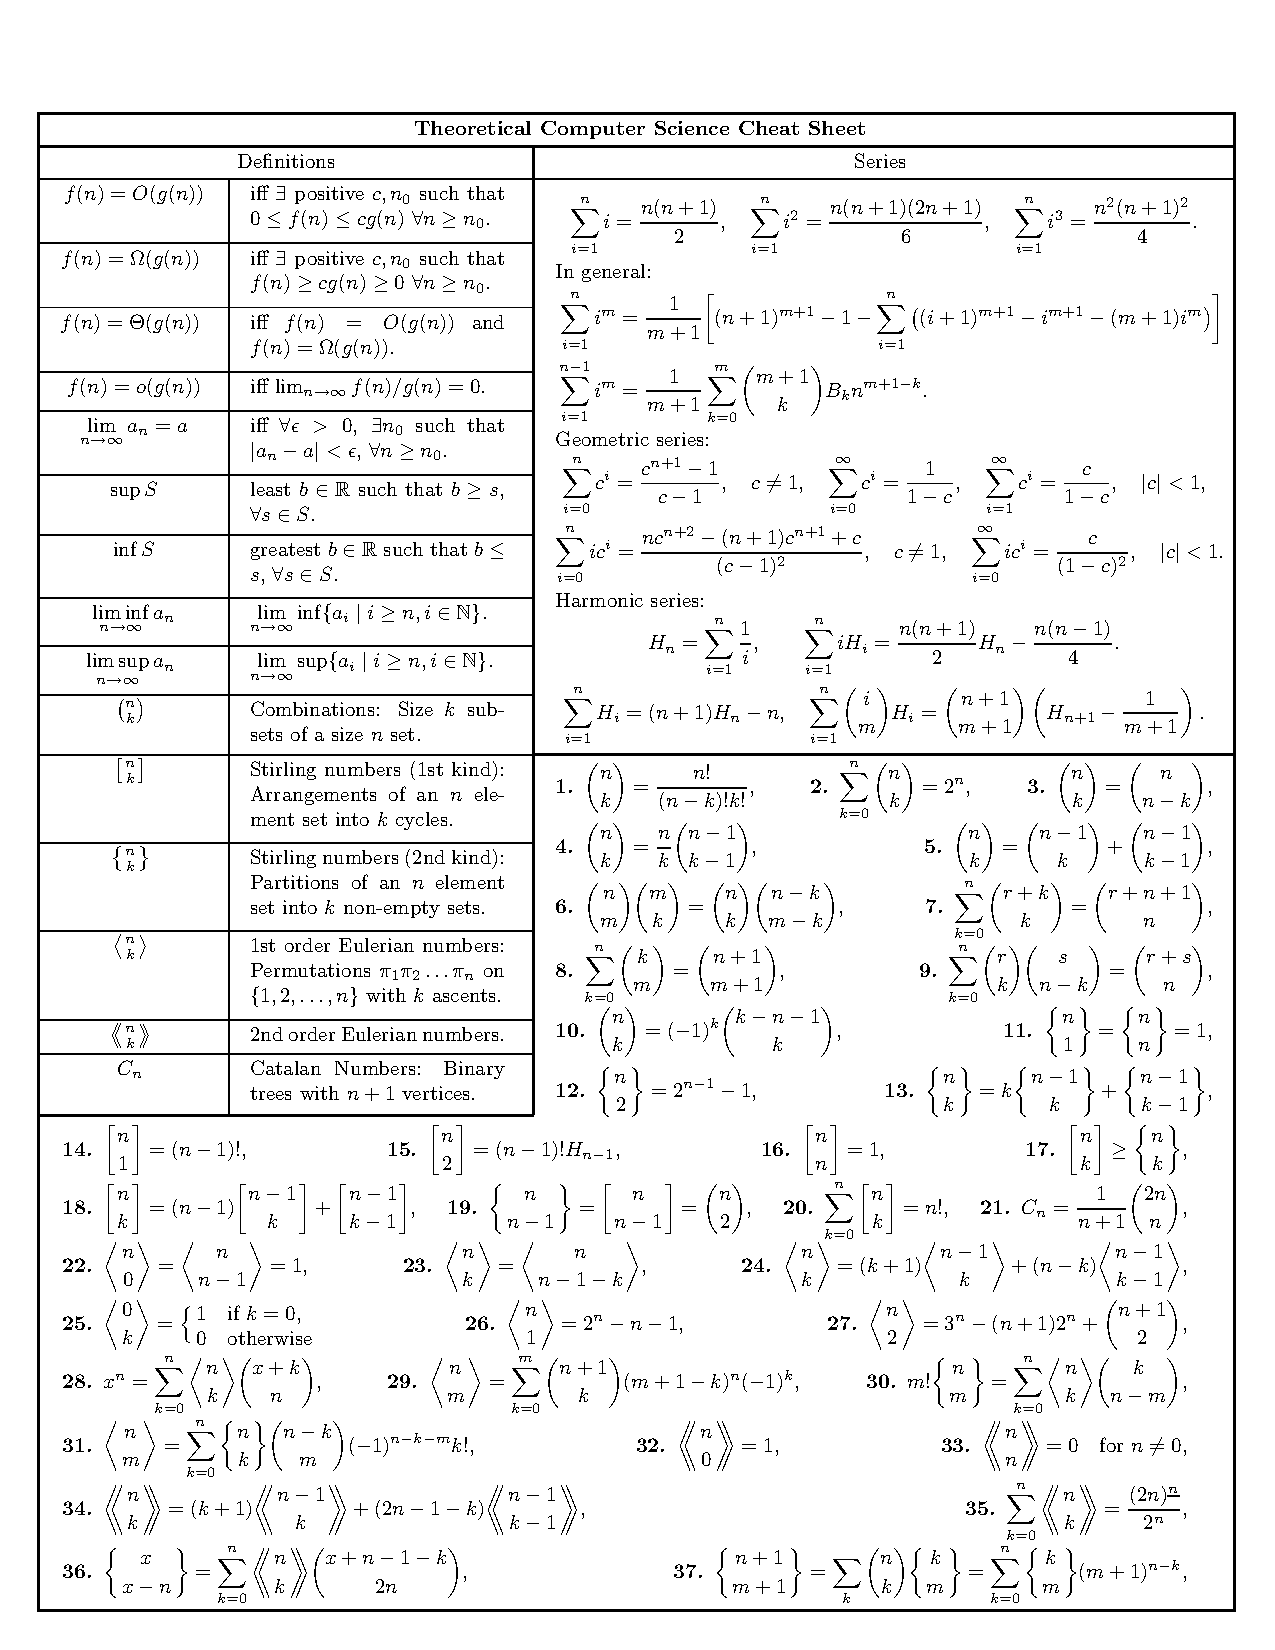
\includepdf[pages=-,pagecommand={}]{src/src/cheat.pdf}

\bibliographystyle{plain}
\bibliography{notebook}
\end{document}
